% Options for packages loaded elsewhere
% Options for packages loaded elsewhere
\PassOptionsToPackage{unicode}{hyperref}
\PassOptionsToPackage{hyphens}{url}
\PassOptionsToPackage{dvipsnames,svgnames,x11names}{xcolor}
%
\documentclass[
  13pt,
]{article}
\usepackage{xcolor}
\usepackage[margin=2cm]{geometry}
\usepackage{amsmath,amssymb}
\setcounter{secnumdepth}{5}
\usepackage{iftex}
\ifPDFTeX
  \usepackage[T1]{fontenc}
  \usepackage[utf8]{inputenc}
  \usepackage{textcomp} % provide euro and other symbols
\else % if luatex or xetex
  \usepackage{unicode-math} % this also loads fontspec
  \defaultfontfeatures{Scale=MatchLowercase}
  \defaultfontfeatures[\rmfamily]{Ligatures=TeX,Scale=1}
\fi
\usepackage{lmodern}
\ifPDFTeX\else
  % xetex/luatex font selection
  \setmainfont[]{Times New Roman}
\fi
% Use upquote if available, for straight quotes in verbatim environments
\IfFileExists{upquote.sty}{\usepackage{upquote}}{}
\IfFileExists{microtype.sty}{% use microtype if available
  \usepackage[]{microtype}
  \UseMicrotypeSet[protrusion]{basicmath} % disable protrusion for tt fonts
}{}
\usepackage{setspace}
\makeatletter
\@ifundefined{KOMAClassName}{% if non-KOMA class
  \IfFileExists{parskip.sty}{%
    \usepackage{parskip}
  }{% else
    \setlength{\parindent}{0pt}
    \setlength{\parskip}{6pt plus 2pt minus 1pt}}
}{% if KOMA class
  \KOMAoptions{parskip=half}}
\makeatother
% Make \paragraph and \subparagraph free-standing
\makeatletter
\ifx\paragraph\undefined\else
  \let\oldparagraph\paragraph
  \renewcommand{\paragraph}{
    \@ifstar
      \xxxParagraphStar
      \xxxParagraphNoStar
  }
  \newcommand{\xxxParagraphStar}[1]{\oldparagraph*{#1}\mbox{}}
  \newcommand{\xxxParagraphNoStar}[1]{\oldparagraph{#1}\mbox{}}
\fi
\ifx\subparagraph\undefined\else
  \let\oldsubparagraph\subparagraph
  \renewcommand{\subparagraph}{
    \@ifstar
      \xxxSubParagraphStar
      \xxxSubParagraphNoStar
  }
  \newcommand{\xxxSubParagraphStar}[1]{\oldsubparagraph*{#1}\mbox{}}
  \newcommand{\xxxSubParagraphNoStar}[1]{\oldsubparagraph{#1}\mbox{}}
\fi
\makeatother


\usepackage{longtable,booktabs,array}
\usepackage{calc} % for calculating minipage widths
% Correct order of tables after \paragraph or \subparagraph
\usepackage{etoolbox}
\makeatletter
\patchcmd\longtable{\par}{\if@noskipsec\mbox{}\fi\par}{}{}
\makeatother
% Allow footnotes in longtable head/foot
\IfFileExists{footnotehyper.sty}{\usepackage{footnotehyper}}{\usepackage{footnote}}
\makesavenoteenv{longtable}
\usepackage{graphicx}
\makeatletter
\newsavebox\pandoc@box
\newcommand*\pandocbounded[1]{% scales image to fit in text height/width
  \sbox\pandoc@box{#1}%
  \Gscale@div\@tempa{\textheight}{\dimexpr\ht\pandoc@box+\dp\pandoc@box\relax}%
  \Gscale@div\@tempb{\linewidth}{\wd\pandoc@box}%
  \ifdim\@tempb\p@<\@tempa\p@\let\@tempa\@tempb\fi% select the smaller of both
  \ifdim\@tempa\p@<\p@\scalebox{\@tempa}{\usebox\pandoc@box}%
  \else\usebox{\pandoc@box}%
  \fi%
}
% Set default figure placement to htbp
\def\fps@figure{htbp}
\makeatother


% definitions for citeproc citations
\NewDocumentCommand\citeproctext{}{}
\NewDocumentCommand\citeproc{mm}{%
  \begingroup\def\citeproctext{#2}\cite{#1}\endgroup}
\makeatletter
 % allow citations to break across lines
 \let\@cite@ofmt\@firstofone
 % avoid brackets around text for \cite:
 \def\@biblabel#1{}
 \def\@cite#1#2{{#1\if@tempswa , #2\fi}}
\makeatother
\newlength{\cslhangindent}
\setlength{\cslhangindent}{1.5em}
\newlength{\csllabelwidth}
\setlength{\csllabelwidth}{3em}
\newenvironment{CSLReferences}[2] % #1 hanging-indent, #2 entry-spacing
 {\begin{list}{}{%
  \setlength{\itemindent}{0pt}
  \setlength{\leftmargin}{0pt}
  \setlength{\parsep}{0pt}
  % turn on hanging indent if param 1 is 1
  \ifodd #1
   \setlength{\leftmargin}{\cslhangindent}
   \setlength{\itemindent}{-1\cslhangindent}
  \fi
  % set entry spacing
  \setlength{\itemsep}{#2\baselineskip}}}
 {\end{list}}
\usepackage{calc}
\newcommand{\CSLBlock}[1]{\hfill\break\parbox[t]{\linewidth}{\strut\ignorespaces#1\strut}}
\newcommand{\CSLLeftMargin}[1]{\parbox[t]{\csllabelwidth}{\strut#1\strut}}
\newcommand{\CSLRightInline}[1]{\parbox[t]{\linewidth - \csllabelwidth}{\strut#1\strut}}
\newcommand{\CSLIndent}[1]{\hspace{\cslhangindent}#1}



\setlength{\emergencystretch}{3em} % prevent overfull lines

\providecommand{\tightlist}{%
  \setlength{\itemsep}{0pt}\setlength{\parskip}{0pt}}



 


\usepackage{booktabs}
\usepackage{longtable}
\usepackage{array}
\usepackage{multirow}
\usepackage{wrapfig}
\usepackage{float}
\usepackage{colortbl}
\usepackage{pdflscape}
\usepackage{tabu}
\usepackage{threeparttable}
\usepackage{threeparttablex}
\usepackage[normalem]{ulem}
\usepackage{makecell}
\usepackage{xcolor}
\usepackage[noblocks]{authblk}
\renewcommand*{\Authsep}{, }
\renewcommand*{\Authand}{, }
\renewcommand*{\Authands}{, }
\renewcommand\Affilfont{\small}
\makeatletter
\@ifpackageloaded{caption}{}{\usepackage{caption}}
\AtBeginDocument{%
\ifdefined\contentsname
  \renewcommand*\contentsname{Table of contents}
\else
  \newcommand\contentsname{Table of contents}
\fi
\ifdefined\listfigurename
  \renewcommand*\listfigurename{List of Figures}
\else
  \newcommand\listfigurename{List of Figures}
\fi
\ifdefined\listtablename
  \renewcommand*\listtablename{List of Tables}
\else
  \newcommand\listtablename{List of Tables}
\fi
\ifdefined\figurename
  \renewcommand*\figurename{Figure}
\else
  \newcommand\figurename{Figure}
\fi
\ifdefined\tablename
  \renewcommand*\tablename{Table}
\else
  \newcommand\tablename{Table}
\fi
}
\@ifpackageloaded{float}{}{\usepackage{float}}
\floatstyle{ruled}
\@ifundefined{c@chapter}{\newfloat{codelisting}{h}{lop}}{\newfloat{codelisting}{h}{lop}[chapter]}
\floatname{codelisting}{Listing}
\newcommand*\listoflistings{\listof{codelisting}{List of Listings}}
\makeatother
\makeatletter
\makeatother
\makeatletter
\@ifpackageloaded{caption}{}{\usepackage{caption}}
\@ifpackageloaded{subcaption}{}{\usepackage{subcaption}}
\makeatother
\usepackage{bookmark}
\IfFileExists{xurl.sty}{\usepackage{xurl}}{} % add URL line breaks if available
\urlstyle{same}
\hypersetup{
  pdftitle={Stability and comparability of meritocratic beliefs in school-age students: A measurement invariance approach across time and cohorts},
  colorlinks=true,
  linkcolor={blue},
  filecolor={Maroon},
  citecolor={Blue},
  urlcolor={Blue},
  pdfcreator={LaTeX via pandoc}}


\title{Stability and comparability of meritocratic beliefs in school-age
students: A measurement invariance approach across time and cohorts}



\date{}
\begin{document}
\maketitle
\begin{abstract}
Meritocratic beliefs shape how adolescents understand inequality and the
legitimacy of social arrangements. Schools are key sites of meritocratic
socialization, making adolescence a crucial period for studying how
these beliefs are formed. However, research on adolescents' meritocratic
beliefs has often relied on unidimensional measures that conflate
perceptions of how allocation works with preferences about how it should
work and treat meritocratic and non-meritocratic principles as
opposites. This study tests a multidimensional model that distinguishes
between perceived and preferred meritocracy and non-meritocracy. Using
two-wave panel survey data from Chilean students in 8th and 10th grade
(Wave 1: N = 846; Wave 2: N = 662), we assess whether these dimensions
can be distinguished, compared across school stages, and measured
equivalently over time. Results support a four-factor structure and show
that endorsement of merit can coexist with recognition of
non-meritocratic advantage. The scale achieves strict longitudinal
invariance within students but not across school levels. \newline
\textbf{Keywords}: Meritocracy · Schools · Measurement invariance ·
Socialization · Chile
\end{abstract}


\setstretch{1.5}
\section{Introduction}\label{introduction}

Despite rising economic inequality and limited social mobility in
contemporary societies (\citeproc{ref-chancel_world_2025}{Chancel et
al., 2025}; \citeproc{ref-lopez-roldan_comparative_2021}{López-Roldán \&
Fachelli, 2021}), the belief that inequalities reflect disparities in
effort and talent instead of opportunities remains remarkably widespread
among citizens (\citeproc{ref-mijs_paradox_2021}{Mijs, 2021}). This idea
refers to meritocracy, the notion that social rewards are, and should
be, allocated according to individual effort and ability rather than
social origins or personal connections
(\citeproc{ref-young_rise_1958}{Young, 1958}). Although the term
``meritocracy'' was originally coined as a critique of a future society
where meritocratic principles would be taken to an extreme
(\citeproc{ref-young_rise_1958}{Young, 1958}), it has since been widely
adopted as a normative ideal that justifies existing social arrangements
and motivates individual striving
(\citeproc{ref-mijs_paradox_2021}{Mijs, 2021};
\citeproc{ref-sandel_tyranny_2020}{Sandel, 2020}). On the one hand,
meritocracy can be seen as a powerful narrative that promotes social
cohesion and motivates individuals to work hard and pursue their goals.
On the other hand, it can also be criticized for obscuring structural
inequalities and legitimizing the status quo
(\citeproc{ref-mijs_paradox_2021}{Mijs, 2021};
\citeproc{ref-sandel_tyranny_2020}{Sandel, 2020}). Therefore, the
persistence of meritocratic beliefs could have important implications
for how people understand and respond to inequality, as well as for the
legitimacy of social institutions
(\citeproc{ref-madeira_primes_2019}{Madeira et al., 2019};
\citeproc{ref-sandel_tyranny_2020}{Sandel, 2020}).

The idea of meritocracy is particularly salient in school settings,
where it operates not only as a cultural ideal but also as a central
organizing principle of institutional life. Schools promote meritocracy
as a normative standard by presenting education as a legitimate pathway
to upward mobility and by framing individual effort and achievement as
the proper basis of social rewards
(\citeproc{ref-lampert_meritocratic_2013}{Lampert, 2013};
\citeproc{ref-vandewerfhorst_meritocracy_2024}{Van De Werfhorst, 2024}).
In this environment, students encounter meritocracy not only as
discourse but also as a lived experience through grading, selection, and
tracking, which make merit visible and consequential
(\citeproc{ref-darnon_where_2018}{Darnon et al., 2018};
\citeproc{ref-resh_sense_2014}{Resh \& Sabbagh, 2014};
\citeproc{ref-tang_meritocratic_2025}{Tang et al., 2025};
\citeproc{ref-traini_stratification_2022}{Traini, 2022}). In this same
socialization process, students are also exposed to non-meritocratic
factors, such as the influence of family background, social connections,
and structural barriers, which may coexist with or undermine the
meritocratic ideal (\citeproc{ref-bourdieu_reproduction_1990}{Bourdieu
\& Passeron, 1990}; \citeproc{ref-goudeau_hidden_2017a}{Goudeau \&
Croizet, 2017}; \citeproc{ref-zhou_equalization_2019}{Zhou, 2019}). In
this line, extant research shows that a stronger endorsement of
meritocratic beliefs in school is associated with greater justification
of inequality (\citeproc{ref-batruch_belief_2022}{Batruch et al., 2022};
\citeproc{ref-lampert_meritocratic_2013}{Lampert, 2013};
\citeproc{ref-wiederkehr_belief_2015}{Wiederkehr et al., 2015}), even
when students may simultaneously recognize structural constraints,
reflecting a form of dual consciousness (\citeproc{ref-liu_does_2025}{C.
Liu \& Wang, 2025}). Taken together, these tensions make schools a
crucial setting for examining how adolescents understand meritocracy,
non-meritocratic constraints, and the fairness of unequal outcomes.

The present paper contributes to this line of research by examining how
school-aged students perceive and endorse meritocracy. We identify two
main contributions of this study. The first one is the conceptualization
and measurement of meritocratic beliefs in school settings. Most of the
research in this area has focused on the consequences of meritocratic
beliefs, while less attention has been paid to their conceptualization
and measurement. This is a crucial gap in the extant literature, as how
meritocratic beliefs are conceptualized and measured can have important
implications for the validity of research findings and their
interpretation. Addressing this point, we approach the study of
meritocratic beliefs at school from a multidimensional approach
(\citeproc{ref-castillo_multidimensional_2023}{Castillo et al., 2023}),
which distinguishes between perceptions (descriptive beliefs about how
meritocracy works) and preferences (normative beliefs about how it
should work), as well as between meritocratic principles (e.g., effort
and ability) and non-meritocratic principles (e.g., family background
and social connections). By adopting this perspective, we can better
capture the complexity of adolescents' beliefs about meritocracy and the
role schools play in fostering them.

A second contribution of this study is to examine the stability and
comparability of meritocratic beliefs across school stages and over
time. Most research on meritocratic beliefs remains cross-sectional,
limiting what we can infer about how these orientations develop through
school-based socialization during adolescence. This matters because
adolescence is precisely when reasoning about justice and inequality
becomes more sophisticated and when school-based sorting mechanisms
become increasingly salient (\citeproc{ref-henry_development_2006}{Henry
\& Saul, 2006}; \citeproc{ref-resh_sense_2014}{Resh \& Sabbagh, 2014}),
potentially reshaping how students interpret meritocratic narratives in
light of lived constraints (\citeproc{ref-allen_top_2016}{Allen, 2016}).
To address this, we test measurement invariance across two cohorts of
Chilean secondary students (8th and 10th graders) and longitudinally
within the same students across two waves (2023--2024). Establishing
invariance is essential for valid comparisons: without it, observed
differences across cohorts or over time may reflect changes in how items
are understood and used rather than substantive change in the underlying
constructs (\citeproc{ref-putnick_measurement_2016}{Putnick \&
Bornstein, 2016}; \citeproc{ref-vandeschoot_checklist_2012}{Van De
Schoot et al., 2012}; \citeproc{ref-vandeschoot_editorial_2015}{Van De
Schoot et al., 2015}). By providing this measurement foundation, the
study clarifies whether apparent differences in meritocratic beliefs
reflect genuine developmental change or measurement non-equivalence, and
it strengthens subsequent analyses of how these beliefs relate to
different attitudes toward inequality and social mobility.

According to these two contributions, the research questions guiding
this study are as follows:

\begin{enumerate}
\def\labelenumi{(\arabic{enumi})}
\item
  Do school-aged students distinguish between meritocratic and
  non-meritocratic principles, as well as between perceptions (``what
  is'') and preferences (``what should be'')?
\item
  Can these dimensions be measured in ways that are comparable across
  age cohorts and stable over time?
\end{enumerate}

We argue that a multidimensional conception of meritocratic beliefs
clarifies what adolescents actually endorse---descriptions, ideals, or
both---and provides a stronger basis for valid developmental and
longitudinal analysis. In the following sections, we first review the
literature on meritocratic beliefs in school settings, highlighting the
conceptual and methodological gaps that this study aims to address.
Then, we present the methodology of our study, including the sample,
measures, and analytical strategy. Finally, we discuss the implications
of our findings for understanding adolescents' beliefs about meritocracy
and the consequences of these beliefs for attitudes toward inequality.

\section{Theoretical and empirical
background}\label{theoretical-and-empirical-background}

\subsection{What is meritocracy, and how is it
measured?}\label{what-is-meritocracy-and-how-is-it-measured}

Meritocracy refers to a distributive system in which individual
merit---typically effort and ability---is treated as the main criterion
for allocating rewards, rather than social origins or inherited
privilege (\citeproc{ref-bell_equality_1972}{Bell, 1972};
\citeproc{ref-young_rise_1958}{Young, 1958}). Although Young
(\citeproc{ref-young_rise_1958}{1958}) introduced the term as a
dystopian critique, it has since been reappropriated as a positive ideal
of fairness, especially in liberal and market-oriented societies
(\citeproc{ref-mijs_paradox_2021}{Mijs, 2021};
\citeproc{ref-vandewerfhorst_meritocracy_2024}{Van De Werfhorst, 2024}).
Sociologically, meritocracy operates both as a cognitive judgment about
how inequality works and as a moral lens through which inequality is
evaluated (\citeproc{ref-castillo_meritocracia_2019}{Castillo et al.,
2019}; \citeproc{ref-heuer_legitimizing_2020}{Heuer et al., 2020}).
Precisely because it frames outcomes as earned, however, it can also
reinforce inequality by encouraging winners to see their position as
deserved and losers to internalize failure rather than question
structural conditions
(\citeproc{ref-garcia-sierra_dark_2023}{García-Sierra, 2023};
\citeproc{ref-mijs_stratified_2016}{Mijs, 2016a};
\citeproc{ref-sandel_tyranny_2020}{Sandel, 2020}).

Research on adults has examined both the determinants and consequences
of meritocratic perceptions. Higher-status and upwardly mobile
individuals are more likely to endorse merit-based explanations of
social outcomes (\citeproc{ref-duru-bellat_whos_2012}{Duru-Bellat \&
Tenret, 2012};
\citeproc{ref-garcia-sanchez_perceptions_2018}{García-Sánchez et al.,
2018}; \citeproc{ref-mijs_belief_2022}{Mijs et al., 2022};
\citeproc{ref-traini_climbing_2025}{Traini et al., 2025}), whereas
perceiving society as meritocratic is associated with lower support for
redistribution, greater acceptance of inequality, and stronger
endorsement of market-based allocation
(\citeproc{ref-castillo_perceptions_2025}{Castillo et al., 2025},
\citeproc{ref-castillo_meritocracia_2019}{2019};
\citeproc{ref-hoyt_mindsets_2023}{Hoyt et al., 2023};
\citeproc{ref-paneda-fernandez_relevance_2026}{Pañeda-Fernández et al.,
2026}; \citeproc{ref-tejero-peregrina_perceived_2025}{Tejero-Peregrina
et al., 2025}). Experimental evidence is consistent with a causal
pathway in which upward-mobility or self-made narratives strengthen
meritocratic perceptions and reduce redistributive support, while
downward-mobility cues produce the opposite pattern
(\citeproc{ref-deng_its_2025}{Deng \& Wang, 2025};
\citeproc{ref-matamoros-lima_social_2025}{Matamoros-Lima et al., 2025}).
Overall, this literature suggests that meritocratic perceptions are
systematically linked to both social position and orientations toward
inequality.

This research agenda faces important conceptual and measurement
challenges. Some studies define meritocracy narrowly, often reducing it
to effort or simplified readings of Young's formulation
(\citeproc{ref-mijs_paradox_2021}{Mijs, 2021};
\citeproc{ref-wiederkehr_belief_2015}{Wiederkehr et al., 2015};
\citeproc{ref-young_rise_1958}{Young, 1958}), while others blur it with
broader constructs such as system justification, beliefs about mobility,
or support for equal opportunity
(\citeproc{ref-batruch_belief_2022}{Batruch et al., 2022};
\citeproc{ref-darnon_where_2018}{Darnon et al., 2018};
\citeproc{ref-day_movin_2017}{Day \& Fiske, 2017};
\citeproc{ref-deng_its_2025}{Deng \& Wang, 2025};
\citeproc{ref-jost_decade_2004a}{Jost et al., 2004};
\citeproc{ref-mccoy_priming_2007}{McCoy \& Major, 2007}). As a result,
conceptually distinct orientations are often collapsed into a single
indicator, and the distinction between descriptive perceptions of how
rewards are allocated and normative preferences about how they should be
allocated is acknowledged but rarely implemented analytically.

A related limitation concerns the treatment of non-meritocratic factors
such as family wealth, social connections, or inherited advantage. As
Castillo et al. (\citeproc{ref-castillo_multidimensional_2023}{2023})
notes, many studies ask respondents to rate the importance of
meritocratic and non-meritocratic factors for ``getting ahead,'' but
then collapse them into a single score. This is especially problematic
when researchers treat both as opposite ends of the same continuum, for
example, through subtraction scores
(\citeproc{ref-reynolds_perceptions_2014a}{Reynolds \& Xian, 2014}).
Such measures impose a zero-sum assumption---namely, that endorsing
merit implies rejecting structural or relational advantages---and
therefore rule out the possibility that both beliefs coexist. Recent
debates and empirical evidence suggest the opposite: support for merit
can coexist with recognition of privilege, contacts, or structural
constraints (\citeproc{ref-kwon_multidimensionality_2024}{Kwon \&
Pandian, 2024}; \citeproc{ref-liu_does_2025}{C. Liu \& Wang, 2025};
\citeproc{ref-mijs_visualizing_2026}{Mijs, 2026};
\citeproc{ref-tang_meritocratic_2025}{Tang et al., 2025};
\citeproc{ref-wiesner_effort_2026}{Wiesner \& Sachweh, 2026};
\citeproc{ref-zhu_meritocratic_2025}{Zhu, 2025}). The implication is
clear: unidimensional indices, especially subtraction scores, can
obscure substantively distinct belief profiles.

Responding to these limitations, Castillo et al.
(\citeproc{ref-castillo_multidimensional_2023}{2023}) proposed a
multidimensional framework that distinguishes meritocratic beliefs along
two analytically independent axes: perceptions versus preferences, and
meritocratic versus non-meritocratic allocation principles. Preferences
capture normative ideals about how rewards should be distributed,
whereas perceptions capture descriptive evaluations of how society
actually works (\citeproc{ref-janmaat_subjective_2013}{Janmaat, 2013}).
At the same time, meritocratic elements (e.g., effort, talent) and
non-meritocratic elements (e.g., social origins, inherited privilege,
networks) are treated as distinct components rather than opposite poles
of a single continuum. This yields four non-redundant
constructs---meritocratic preferences, meritocratic perceptions,
non-meritocratic preferences, and non-meritocratic perceptions---and
allows combinations that older measures collapse, such as endorsing
meritocracy as an ideal while recognizing the role of family background
and connections. The framework is also parsimonious and therefore well
suited to large-scale surveys, although its reliance on only two items
per factor may constrain reliability and content coverage.

Evidence from adult samples using confirmatory factor analysis suggests
that respondents can differentiate among these four dimensions and that
they are systematically related. In particular, stronger perceptions
that non-meritocratic factors are rewarded tend to coexist with stronger
preferences for meritocratic allocation. This pattern aligns with Zhu's
(\citeproc{ref-zhu_meritocratic_2025}{2025}) notion of ``dual
consciousness,'' understood here as the coexistence of meritocratic and
non-meritocratic beliefs, as well as descriptive assessments (``is'')
and legitimacy judgments (``should'').

In school research, these measurement challenges have received little
attention. One recent exception is Chauvin et al.
(\citeproc{ref-chauvin_school_2026}{2026}), who proposes a
multidimensional measure of school meritocracy, but it applies only to
teachers and remains limited to perceived meritocracy. Another relevant
study, by Castillo et al.
(\citeproc{ref-castillo_socialization_2024}{2024}), applies the
multidimensional framework to Chilean 10th graders and shows that
students can differentiate between perceptions and preferences, as well
as between meritocratic and non-meritocratic principles. However, that
study does not examine whether these dimensions are stable across
cohorts or over time, limiting our understanding of their developmental
trajectory and comparability.

\subsection{The socialization of meritocracy at
school}\label{the-socialization-of-meritocracy-at-school}

Socialization refers to the process through which individuals
internalize norms, values, and practices, acquiring the dispositions
needed to function in society. From a sociological perspective, this
process is neither neutral nor purely individual, but structured by
relations of power and inequality
(\citeproc{ref-bourdieu_sentido_2007}{Bourdieu, 2007}). Likewise, social
learning approaches emphasize that children adopt behavioral patterns
and value systems modeled in their everyday environments, especially
within families (\citeproc{ref-bandura_sociallearning_1969}{Bandura,
1969}). The internalization of meritocratic beliefs---such as the idea
that effort and talent determine success---should therefore be
understood not as a purely rational judgment but as the outcome of
structured, socially differentiated socialization processes.

Families play a foundational role in early meritocratic orientations.
Parenting often reflects class-based strategies of status reproduction
(\citeproc{ref-bernstein_theoretical_2005}{Bernstein, 2005};
\citeproc{ref-bourdieu_reproduction_1990}{Bourdieu \& Passeron, 1990}),
and children internalize parental views of success, fairness, and
responsibility through everyday interactions
(\citeproc{ref-bandura_sociallearning_1969}{Bandura, 1969}). Yet schools
constitute a particularly consequential institutional arena in which
these beliefs are further shaped, reinforced, and contested.

Schools socialize meritocracy both culturally and institutionally. They
promote narratives of effort, achievement, self-improvement, and
education as a legitimate route to mobility
(\citeproc{ref-batruch_belief_2022}{Batruch et al., 2022};
\citeproc{ref-chauvin_school_2026}{Chauvin et al., 2026};
\citeproc{ref-darnon_where_2018}{Darnon et al., 2018};
\citeproc{ref-mijs_paradox_2021}{Mijs, 2021};
\citeproc{ref-wiederkehr_belief_2015}{Wiederkehr et al., 2015}), while
embedding these ideals in routine practices of evaluation and
classification such as grading, tracking, selection, awards, and
credentials (\citeproc{ref-resh_sense_2014}{Resh \& Sabbagh, 2014};
\citeproc{ref-traini_stratification_2022}{Traini, 2022}). At the same
time, schools are settings where non-meritocratic advantages---such as
family resources, cultural capital, peer environments, and unequal
school quality---also become visible and consequential
(\citeproc{ref-batruch_belief_2022}{Batruch et al., 2022};
\citeproc{ref-resh_sense_2014}{Resh \& Sabbagh, 2014}). This duality
makes educational settings especially important for understanding how
meritocratic beliefs are formed.

A growing literature shows that this duality can generate internally
differentiated orientations. Students may endorse meritocracy as a
normative ideal while simultaneously recognizing structural constraints,
a pattern described as ``dual consciousness''
(\citeproc{ref-liu_does_2025}{C. Liu \& Wang, 2025};
\citeproc{ref-tang_meritocratic_2025}{Tang et al., 2025}). More broadly,
meritocratic framing encourages students to interpret success and
failure in individual terms, reinforcing personal responsibility while
limiting attention to structural conditions
(\citeproc{ref-darnon_where_2018}{Darnon et al., 2018};
\citeproc{ref-lampert_meritocratic_2013}{Lampert, 2013}). Even
disadvantaged students often adopt meritocratic narratives, suggesting
that prolonged exposure to school-based evaluative environments is a
powerful mechanism shaping beliefs about justice and inequality
(\citeproc{ref-henry_development_2006}{Henry \& Saul, 2006}).

These beliefs matter beyond school. Perceiving schools as
meritocratic---particularly believing that effort and talent are fairly
rewarded---has been linked to greater legitimation of inequality,
including stronger system justification, lower support for
redistribution, and greater acceptance of unequal access to key social
services (\citeproc{ref-batruch_belief_2022}{Batruch et al., 2022};
\citeproc{ref-castillo_socialization_2024}{Castillo et al., 2024};
\citeproc{ref-wiederkehr_belief_2015}{Wiederkehr et al., 2015}). Schools
thus shape not only academic trajectories, but also early distributive
beliefs that may normalize broader social inequalities.

\subsection{This study}\label{this-study}

This study examines how students understand meritocracy during a
formative stage of socialization---schooling---and whether these
understandings can be measured reliably and comparably. Building on
Castillo et al.'s (\citeproc{ref-castillo_multidimensional_2023}{2023})
conceptual and measurement framework, we test whether students
differentiate between perceptions of how meritocracy operates (``what
is'') and preferences about how it should operate (``what ought to
be''), and whether these judgments distinguish meritocratic elements
(effort, talent) from non-meritocratic ones (family wealth, personal
contacts). Beyond factorial validity, the paper focuses on measurement
stability---whether the same latent constructs are captured comparably
across school stages and over time within the same students.

Establishing measurement invariance is essential because it provides the
empirical foundation for valid comparisons
(\citeproc{ref-chen_sensitivity_2007}{Chen, 2007};
\citeproc{ref-putnick_measurement_2016}{Putnick \& Bornstein, 2016}).
Without it, observed differences between groups or across time may
reflect changes in how the instrument functions rather than substantive
differences in the underlying constructs
(\citeproc{ref-putnick_measurement_2016}{Putnick \& Bornstein, 2016};
\citeproc{ref-vandeschoot_editorial_2015}{Van De Schoot et al., 2015}).
In sociological terms, invariance matters because comparisons are only
interpretable if a given latent score carries the same meaning across
ages or time points; otherwise, apparent developmental or group
differences may conflate substantive variation with measurement
artifacts (\citeproc{ref-liu_testing_2017}{Y. Liu et al., 2017};
\citeproc{ref-vandeschoot_checklist_2012}{Van De Schoot et al., 2012}).

The study uses longitudinal data from two cohorts of Chilean secondary
students: 8th graders (approximately 12--13 years old) and 10th graders
(approximately 15--16 years old) at baseline, followed across two waves.
These cohorts are theoretically strategic because they capture distinct
stages of adolescence, when reasoning about justice and inequality
becomes more sophisticated and school-based sorting mechanisms---grades,
tracking, and peer comparisons---become increasingly salient
(\citeproc{ref-henry_development_2006}{Henry \& Saul, 2006};
\citeproc{ref-resh_sense_2014}{Resh \& Sabbagh, 2014}). Developmental
research further suggests that by around age 10, children can already
articulate judgments about social differences, often emphasizing
individual, merit-based explanations while beginning to incorporate
opportunity-based accounts (\citeproc{ref-imhoff_nociones_2025}{Imhoff
\& Brussino, 2025}; \citeproc{ref-sigelman_age_2013a}{Sigelman, 2013}).
As students move through the school system, cumulative exposure to
evaluation and selection may make the limits of effort as a sufficient
explanation for success more visible, generating a potential ``reality
shock'' as meritocratic discourse clashes with experienced inequality
and constraint (\citeproc{ref-allen_top_2016}{Allen, 2016}). Both
cohorts are embedded in the same highly stratified educational system,
yet differ in their cumulative exposure to schooling and to the
meritocratic narratives the system promotes. We therefore test
invariance across cohorts and waves to determine whether observed
differences and changes can be interpreted substantively rather than as
artifacts of measurement non-equivalence.

\subsubsection{Hypotheses}\label{hypotheses}

\textbf{\(H_1\) (Dimensional differentiation)}. Students' meritocratic
beliefs are best represented by four distinct factors: perceived
meritocracy, perceived non-meritocracy, preferred meritocracy, and
preferred non-meritocracy.

\textbf{\(H_2\) (Between-cohort measurement invariance)}. The
four-factor model of meritocratic beliefs is invariant across age
cohorts.

\textbf{\(H_3\) (Longitudinal measurement invariance)}. The four-factor
model of meritocratic beliefs is invariant across waves within students.

\section{Method}\label{method}

\subsection{Participants}\label{participants}

This study uses secondary data from the 2023 and 2024 waves of the Panel
Survey on Education and Meritocracy (EDUMER), which examines school-age
students' beliefs, attitudes, and behaviors regarding meritocracy,
inequality, and citizenship\footnote{The survey was collected within the
  research project ``Meritocracy in schools: Moral foundations of the
  education market and its implications for civic education in Chile''
  (FONDECYT Regular 2021 Nº 1210847).}. The questionnaire was
administered to sixth-grade and first-year secondary students in nine
schools in Chile's Metropolitan and Valparaíso regions. Although the
sample was non-probabilistic and lacked quota controls, a minimum target
of 900 students was set to ensure adequate statistical power. After data
processing and listwise deletion, the analytical sample included 846
students in Wave 1 (386 girls, 421 boys, 39 identifying as other;
\(M_{age}\) = 13.4, \(SD_{age}\) = 1.6) and 662 in Wave 2 (303 girls,
338 boys, 21 identifying as other; \(M_{age}\) = 14.4, \(SD_{age}\) =
1.6), yielding a retention rate of 78.3\% (attrition = 21.7\%). The main
sources of attrition were school transfers between academic years and
high absenteeism in several schools.

\subsection{Procedure}\label{procedure}

Data were collected by a professional research firm using online CAWI
questionnaires. All participants received informed consent, which was
reviewed and approved by a parent or legal guardian. To enable
longitudinal linkage while protecting confidentiality, the survey firm
generated anonymous unique identifiers for each student, and no directly
identifying information was included in the analytic files.

\subsection{Measures}\label{measures}

\subsubsection{Scale of perceptions and preferences of
meritocracy}\label{scale-of-perceptions-and-preferences-of-meritocracy}

Meritocratic and non-meritocratic perceptions and preferences were
measured using the same items proposed in the original scale
(\citeproc{ref-castillo_multidimensional_2023}{Castillo et al., 2023}).
Each of the four dimensions of the scale is measured by two items. The
dimensions are:

\begin{itemize}
\item
  Perceived meritocracy: the extent to which effort and ability are
  rewarded in Chile,
\item
  Perceived non-meritocracy: the extent to which success is perceived as
  linked to connections and family wealth,
\item
  Preference for meritocracy: agreement with that those who work harder
  or are more talented should be better rewarded,
\item
  Preference for non-meritocracy: agreement with that it is acceptable
  for individuals with better connections or wealthy parents to achieve
  greater success (see Table~\ref{tbl-merit}).
\end{itemize}

Each item is rated on a four-point Likert scale ranging from ``strongly
disagree'' (1) to ``strongly agree'' (4), therefore higher scores
indicate stronger endorsement of the corresponding perception or
preference.

\begin{table}

\caption{\label{tbl-merit}Items for perceptions and preferences for
meritocracy scale}

\centering{

\begingroup\fontsize{9.5}{11.5}\selectfont

\begin{tabu} to \linewidth {>{\raggedright\arraybackslash}p{2cm}>{\raggedright\arraybackslash}p{2 cm}>{\raggedright}X>{\raggedright}X}
\toprule
Components & Dimensions & Item (English) & Item original (Spanish)\\
\midrule
 &  & In Chile people are rewarded for their efforts & En Chile las personas son recompensadas por sus esfuerzos\\
\cmidrule{3-4}
 & \multirow{-2}{2 cm}{\raggedright\arraybackslash Meritocratic} & In Chile people are rewarded for their intelligence and ability & En Chile las personas son recompensadas por su inteligencia y habilidad\\
\cmidrule{2-4}
 &  & In Chile those with wealthy parents do much better in life & En Chile a quienes tienen padres ricos les va mucho mejor en la vida\\
\cmidrule{3-4}
\multirow{-4}{2cm}[0.5\dimexpr\aboverulesep+\belowrulesep+\cmidrulewidth]{\raggedright\arraybackslash Perception} & \multirow{-2}{2 cm}{\raggedright\arraybackslash Non meritocratic} & In Chile those with good contacts do much better in life & En Chile a quienes tienen buenos contactos les va mejor en la vida\\
\cmidrule{1-4}
 &  & Those who work harder should reap greater rewards than those who work less hard & Quienes más se esfuerzan deberían obtener mayores recompensas que quienes se esfuerzan menos\\
\cmidrule{3-4}
 & \multirow{-2}{2 cm}{\raggedright\arraybackslash Meritocratic} & Those with more talent should reap greater rewards than those with less talent & Quienes poseen más talento deberían obtener mayores recompensas que quienes poseen menos talento\\
\cmidrule{2-4}
 &  & It is good that those who have rich parents do better in life & Está bien que quienes tengan padres ricos les vaya mejor en la vida\\
\cmidrule{3-4}
\multirow{-4}{2cm}[0.5\dimexpr\aboverulesep+\belowrulesep+\cmidrulewidth]{\raggedright\arraybackslash Preference} & \multirow{-2}{2 cm}{\raggedright\arraybackslash Non meritocratic} & It is good that those who have good contacts do better in life & Está bien que quienes tengan buenos contactos les vaya mejor en la vida\\
\bottomrule
\end{tabu}
\endgroup{}

}

\end{table}%

\subsubsection{Cohort level}\label{cohort-level}

To distinguish students' academic level across waves for conditional and
multi-group invariance analyses, we created a cohort indicator capturing
whether the respondent belonged to the primary (sixth grade) or
secondary (first-year secondary) cohort at the time of each survey wave.
Descriptive statistics\footnote{Table~\ref{tbl-cohort} totals (N =
  1,508) correspond to the sum of person-wave observations (846 at T1 +
  662 at T2), rather than unique individuals.} by cohort are reported in
Table~\ref{tbl-cohort}.

\begin{table}

\caption{\label{tbl-cohort}Descriptive statistics for cohort level}

\centering{

\begingroup\fontsize{9.5}{11.5}\selectfont

\begin{tabu} to \linewidth {>{\raggedright}X>{\raggedright}X>{\raggedleft}X>{\raggedleft}X>{\raggedleft}X>{\raggedleft}X>{\raggedleft}X>{\raggedleft}X}
\toprule
\multicolumn{3}{c}{ } & \multicolumn{2}{c}{Age} & \multicolumn{3}{c}{Gender} \\
\cmidrule(l{3pt}r{3pt}){4-5} \cmidrule(l{3pt}r{3pt}){6-8}
Wave & Cohort level & N & Mean & SD & Man & Women & Others\\
\midrule
 & Primary & 406 & 11.85 & 0.56 & 195 & 191 & 20\\
\cmidrule{2-8}
 & Secondary & 440 & 14.79 & 0.80 & 226 & 195 & 19\\
\cmidrule{2-8}
\multirow{-3}{*}{\raggedright\arraybackslash Wave 1} & Total & 846 & 13.38 & 1.63 & 421 & 386 & 39\\
\cmidrule{1-8}
 & Primary & 319 & 12.83 & 0.55 & 161 & 145 & 13\\
\cmidrule{2-8}
 & Secondary & 343 & 15.76 & 0.75 & 177 & 158 & 8\\
\cmidrule{2-8}
\multirow{-3}{*}{\raggedright\arraybackslash Wave 2} & Total & 662 & 14.35 & 1.61 & 338 & 303 & 21\\
\bottomrule
\end{tabu}
\endgroup{}

}

\end{table}%

\subsection{Analytical strategy}\label{analytical-strategy}

\subsubsection{Measurement model and
estimation}\label{measurement-model-and-estimation}

To evaluate the underlying structure of the scale, we employed
Confirmatory Factor Analysis (CFA) based on a measurement model with
four latent factors, using Diagonally Weighted Least Squares with robust
correction (WLSMV) estimation. This estimator is particularly suitable
for ordinal data, such as four-point Likert-type scales, as it avoids
the bias associated with treating categorical data as continuous
(\citeproc{ref-kline_principles_2023}{Kline, 2023}).

Model fit was assessed following the guidelines of Brown
(\citeproc{ref-brown_confirmatory_2015}{2015}), using several indices:
the Comparative Fit Index (CFI) and the Tucker-Lewis Index (TLI), with
acceptable values above 0.95; the Root Mean Square Error of
Approximation (RMSEA), with values below 0.06 indicating good fit; and
the Chi-square statistic (acceptable fit indicated by \(p\)
\textgreater{} 0.05 and a Chi-square/df ratio \textless{} 3).

\subsubsection{Measurement invariance}\label{measurement-invariance}

A key contribution of this study is its assessment of measurement
stability through factorial invariance testing
(\citeproc{ref-davidov_measurement_2014}{Davidov et al., 2014}). We
implemented two complementary strategies: cross-group invariance across
school levels (primary vs.~secondary students) and longitudinal
invariance across two panel waves. Given the ordinal nature of the
items, we used estimation procedures appropriate for ordered categorical
indicators, following Y. Liu et al.
(\citeproc{ref-liu_testing_2017}{2017}) for longitudinal analyses and
Svetina et al. (\citeproc{ref-svetina_multiplegroup_2020}{2020}) for
cross-group tests. We assessed invariance using a hierarchical sequence
of nested confirmatory factor analysis models that imposed progressively
stricter equality constraints. For longitudinal invariance, we estimated
a configural model specifying the same factor structure over time while
allowing item parameters to vary, followed by metric, scalar, and strict
models constraining factor loadings, thresholds/intercepts, and residual
variances, respectively. For cross-group invariance, we estimated a
configural model, then a threshold-invariant model, and finally a model
jointly constraining thresholds and factor loadings across groups.

In addition to the chi-square difference test, we assessed invariance
using changes in approximate fit indices. Following Chen
(\citeproc{ref-chen_sensitivity_2007}{2007}), we treated \(\Delta\)CFI
as the primary criterion and \(\Delta\)RMSEA as supplementary,
indicating noninvariance when \(\Delta\)CFI \(\leq\) −0.010 and
\(\Delta\)RMSEA \(\geq\) 0.015.

All analyses were performed using the \emph{lavaan} package in R version
4.5.2. The hypotheses of this research were
\href{https://osf.io/hjat2/}{pre-registered} on the Open Science
Framework (OSF).

\section{Results}\label{results}

\subsection{Measurement model}\label{measurement-model}

Figure~\ref{fig-general} presents the standardized factor loadings and
the overall fit indices of the general measurement model estimated on
the pooled analytical sample across cohorts and waves. The model shows a
reasonable, though not fully satisfactory, fit to the data (CFI = 0.97;
TLI = 0.94; RMSEA = 0.07). Although the CFI and RMSEA fall within
commonly used acceptable ranges, the TLI remains below conventional
thresholds, indicating that fit is acceptable in some respects but not
uniformly strong across indices. Overall, these results suggest that the
proposed four-factor structure captures the main covariance pattern in
the combined sample reasonably well.

\begin{figure}

\caption{\label{fig-general}Multigroup model diagram}

\centering{

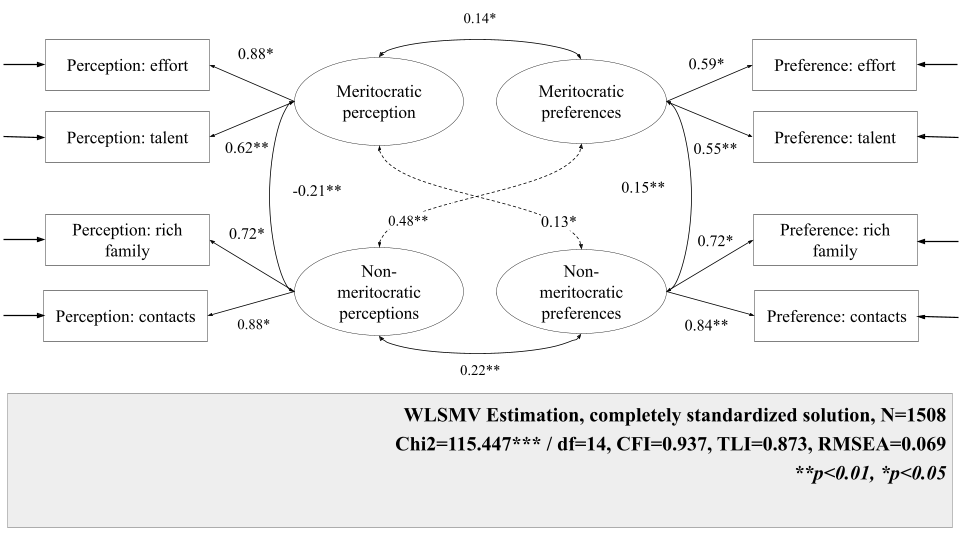
\includegraphics[width=1\linewidth,height=\textheight,keepaspectratio]{../paper/imagenes/esquema-general.png}

}

\end{figure}%

All standardized factor loadings are statistically significant and
generally moderate to strong, though their magnitude varies across
dimensions. For meritocratic perceptions, both indicators load
positively on the latent factor, with effort showing a particularly
strong loading (\(\beta\) = 0.88) and talent a moderately strong loading
(\(\beta\) = 0.62). Meritocratic preferences exhibit more even, but
somewhat weaker, loadings for effort (\(\beta\) = 0.59) and talent
(\(\beta\) = 0.55). For non-meritocratic perceptions, both indicators
load strongly, especially contacts (\(\beta\) = 0.88), followed by
coming from a rich family (\(\beta\) = 0.72). Non-meritocratic
preferences also show strong and relatively balanced loadings, with
contacts (\(\beta\) = 0.84) and rich family (\(\beta\) = 0.72),
indicating that both indicators are similarly representative of this
latent dimension.

The latent correlations reveal a differentiated structure among the four
dimensions. Meritocratic perceptions and meritocratic preferences are
positively correlated (\(r\) = 0.14), consistent with some alignment
between what students perceive is rewarded and what they believe should
be rewarded. Meritocratic and non-meritocratic perceptions are
negatively correlated (\(r\) = −0.21), suggesting that students who
perceive greater meritocracy in society tend to view a weaker role for
connections and family wealth. At the same time, non-meritocratic
perceptions are positively related to meritocratic preferences (\(r\) =
0.48, strongest correlation), suggesting that perceiving society as
rewarding contacts and wealth may coincide with stronger endorsement of
meritocratic ideals. Finally, meritocratic and non-meritocratic
preferences are modestly positively correlated (\(r\) = 0.15), and
non-meritocratic perceptions and preferences are also positively
associated (\(r\) = 0.22), indicating that recognizing non-meritocratic
mechanisms in practice is linked to a greater acceptance of their
legitimacy, albeit to a moderate extent.

\subsection{Invariance analysis}\label{invariance-analysis}

\subsubsection{Longitudinal invariance}\label{longitudinal-invariance}

Figure~\ref{fig-likerplot1} displays the response distributions for the
meritocracy scale, distinguishing perceptions (Panel A) from preferences
(Panel B) across waves. Across both waves, a clear and stable gap
emerges between how students perceive social rewards to operate and how
they think they should operate. In the perception items, agreement is
consistently high for contacts, parental wealth, and talent, whereas
effort is also widely endorsed but to a lesser extent, indicating that
students recognize both meritocratic and non-meritocratic determinants
of success and view talent as more influential than effort. In the
preference items, by contrast, effort is overwhelmingly endorsed as the
legitimate basis for rewards, far exceeding its perceived role in
practice. Talent occupies a more ambivalent normative position, parental
wealth remains evenly divided, and contacts are more often accepted than
rejected, suggesting that non-meritocratic criteria are not uniformly
seen as illegitimate. Wave 2 closely replicates these patterns, with
only modest shifts. Overall, the descriptive results reveal a persistent
paradox: strong endorsement of effort-centered meritocratic ideals
alongside skepticism about their realization in practice.

\begin{figure}

\caption{\label{fig-likerplot1}Distribution of responses on the scale of
perceptions and preferences regarding meritocracy by wave}

\centering{


\includegraphics[width=1\linewidth,height=\textheight,keepaspectratio]{paper_blinded_short_files/figure-pdf/fig-likerplot1-1.pdf}

}

\end{figure}%

Table~\ref{tbl-longinv} reports the results of the longitudinal
invariance tests. Overall, the scale achieved the strongest level of
invariance (strict invariance) across the two waves. The strict model
showed good fit, \(\chi^2\)(84) = 130.17, CFI = 0.991, RMSEA = 0.031
(90\% CI: 0.020--0.040). Moreover, compared with the strong (scalar)
model, the deterioration in fit was negligible: \(\Delta \chi^2\)(4) =
1.635, \(\Delta\)CFI = 0.000, and \(\Delta\)RMSEA = -0.002. These
differences fall well within commonly used cutoffs for invariance
evaluation (\citeproc{ref-chen_sensitivity_2007}{Chen, 2007}),
indicating that constraining residual variances in addition to loadings
and thresholds/intercepts is tenable. Substantively, this implies that
the item--factor relations are stable over time (metric invariance) and
that, for a given level of the latent trait, respondents are expected to
endorse the same response categories across waves (scalar invariance),
supporting the comparability of scores and latent parameters within
students over time.

\begin{table}

\caption{\label{tbl-longinv}Longitudinal invariance results}

\centering{

\begingroup\fontsize{9.5}{11.5}\selectfont

\begin{tabu} to \linewidth {>{\centering\arraybackslash}p{2cm}>{\centering}X>{\centering}X>{\centering\arraybackslash}p{2 cm}>{\centering}X>{\centering}X>{\centering}X>{\centering}X}
\toprule
Model & $\chi^2$ (df) & CFI & RMSEA (90\% CI) & $\Delta \chi^2$ ($\Delta$df) & $\Delta$CFI & $\Delta$RMSEA & Decision\\
\midrule
Configural & 117.7 (68) & 0.991 & 0.035 
 (0.024-0.046) & 0 (0) & 0 & 0.000 & Reference\\
Weak & 122.51 (72) & 0.990 & 0.034 
 (0.024-0.045) & 4.809 (4) & 0 & -0.001 & Accept\\
Strong & 128.53 (80) & 0.991 & 0.032 
 (0.021-0.042) & 6.02 (8) & 0 & -0.002 & Accept\\
Strict & 130.17 (84) & 0.991 & 0.031 
 (0.02-0.04) & 1.635 (4) & 0 & -0.002 & Accept\\
\bottomrule
\end{tabu}
\endgroup{}

}

\end{table}%

As an additional diagnostic, we used univariate score tests to identify
potential sources of localized misfit at each step of the invariance
hierarchy. The tests revealed no meaningful violations of the imposed
equality constraints, suggesting that model fit was not driven by a
small subset of parameters. Global score tests and the smallest p-values
at each step are reported in the supplementary materials.

\subsubsection{Cohort invariance}\label{cohort-invariance}

Figure~\ref{fig-likerplot2} shows response distributions by cohort,
separating perceptions and preferences. In primary education, effort and
talent are perceived as similarly rewarded, while contacts and family
wealth are also seen as advantageous, though with more disagreement. In
secondary education, perceptions become less meritocratic: agreement
that effort is rewarded declines, whereas contacts and family wealth are
seen as more strongly shaping success. Preferences are more stable
across cohorts. In both groups, effort is the most strongly endorsed
legitimate basis for reward, while talent, family wealth, and especially
contacts remain more ambivalent. Notably, contacts are more often
accepted than rejected in both cohorts. Overall, the cohort comparison
reveals a widening gap between an effort-centered meritocratic ideal and
the perceived importance of non-meritocratic advantages in practice.

\begin{figure}

\caption{\label{fig-likerplot2}Distribution of responses on the scale of
perceptions and preferences regarding meritocracy by cohort}

\centering{


\includegraphics[width=1\linewidth,height=\textheight,keepaspectratio]{paper_blinded_short_files/figure-pdf/fig-likerplot2-1.pdf}

}

\end{figure}%

\begin{table}

\caption{\label{tbl-cohort2}Cohort (multigroup) invariance results}

\centering{

\begingroup\fontsize{9.5}{11.5}\selectfont

\begin{tabu} to \linewidth {>{\centering\arraybackslash}p{2cm}>{\centering}X>{\centering}X>{\centering\arraybackslash}p{2 cm}>{\centering\arraybackslash}p{2 cm}>{\centering}X>{\centering}X>{\centering}X}
\toprule
Model & $\chi^2$ (df) & CFI & RMSEA (90\% CI) & $\Delta \chi^2$ ($\Delta$df) & $\Delta$CFI & $\Delta$RMSEA & Decision\\
\midrule
Configural & 24.95 (26) & 0.993 & 0.036 
(0.009-0.057) & 0 (0) & 0.000 & 0.000 & Reference\\
Tresholds & 57.56 (42) & 0.980 & 0.049 
(0.033-0.064) & 43.875 (16) *** & -0.013 & 0.013 & Reject\\
Tresholds + Loadings & 72.35 (46) & 0.973 & 0.053 
(0.039-0.067) & 17.075 (4) ** & -0.006 & 0.005 & Reject\\
\bottomrule
\end{tabu}
\endgroup{}

}

\end{table}%

Table~\ref{tbl-cohort2} summarizes the cross-cohort invariance tests.
The scale achieves configural invariance between primary and secondary
students, but not threshold invariance, and therefore does not meet the
prerequisites for stronger forms of invariance
(\citeproc{ref-svetina_multiplegroup_2020}{Svetina et al., 2020};
\citeproc{ref-wu_identification_2016a}{Wu \& Estabrook, 2016}).
Constraining thresholds worsened model fit (\(\Delta\)CFI = −.013;
\(\Delta\)RMSEA = .013), exceeding recommended cutoffs
(\citeproc{ref-chen_sensitivity_2007}{Chen, 2007}). This indicates that
response categories do not map equivalently onto the latent constructs
across cohorts, limiting direct comparisons of latent means or other
latent differences.

To locate the source of cross-cohort non-invariance, we inspected
localized misfit in the threshold-invariant model. The largest
violations concerned the perceived-effort item, especially the second
threshold (\(\chi^2=10.12, p=.001\)) and, to a lesser extent, the first
(\(\chi^2=7.55, p=.006\)), suggesting that older students may apply a
more critical standard when judging whether effort is rewarded in
society.

\section{Discussion}\label{discussion}

The first hypothesis proposed that students' meritocratic beliefs would
be best represented by four distinct factors: perceived meritocracy,
perceived non-meritocracy, preferred meritocracy, and preferred
non-meritocracy. The confirmatory factor analyses support this
expectation. Consistent with evidence from adult populations
(\citeproc{ref-castillo_multidimensional_2023}{Castillo et al., 2023}),
students already distinguish between perceptions and preferences, and
between meritocratic and non-meritocratic principles at an early stage
of school socialization.

These findings contribute to debates on how meritocratic beliefs should
be conceptualized and measured
(\citeproc{ref-kwon_multidimensionality_2024}{Kwon \& Pandian, 2024};
\citeproc{ref-mijs_visualizing_2026}{Mijs, 2026};
\citeproc{ref-zhu_meritocratic_2025}{Zhu, 2025}). Perceptions of ``what
is'' and preferences about ``what should be'' are empirically separable
among school-aged students, and meritocratic and non-meritocratic
principles coexist rather than forming opposite poles of a single
continuum. This directly challenges zero-sum measurement strategies,
such as subtraction scores, that assume endorsing merit implies
rejecting privilege (\citeproc{ref-reynolds_perceptions_2014a}{Reynolds
\& Xian, 2014}; \citeproc{ref-wiesner_effort_2026}{Wiesner \& Sachweh,
2026}). Instead, our results are more consistent with recent accounts
arguing that recognition of non-meritocratic constraints may increase
without displacing merit ideals (\citeproc{ref-liu_does_2025}{C. Liu \&
Wang, 2025}; \citeproc{ref-tang_meritocratic_2025}{Tang et al., 2025}).
The positive association between perceived non-meritocracy and stronger
meritocratic preferences supports this interpretation, suggesting a
normative-reactive response to perceived unfairness (cf.
\citeproc{ref-castillo_multidimensional_2023}{Castillo et al., 2023}).

The findings also align with research on meritocracy in educational
settings. Schools circulate meritocratic narratives of effort,
achievement, and mobility while institutionalizing merit through
grading, selection, and tracking
(\citeproc{ref-mijs_unfulfillable_2016}{Mijs, 2016b};
\citeproc{ref-resh_sense_2014}{Resh \& Sabbagh, 2014};
\citeproc{ref-tang_meritocratic_2025}{Tang et al., 2025};
\citeproc{ref-traini_climbing_2025}{Traini et al., 2025}). Our results
extend this literature by showing that students not only perceive
meritocracy in multidimensional terms but also differentiate their
preferences and incorporate non-meritocratic considerations. Because
school meritocracy has been linked to inequality legitimation and
broader distributive attitudes
(\citeproc{ref-batruch_belief_2022}{Batruch et al., 2022};
\citeproc{ref-castillo_socialization_2024}{Castillo et al., 2024};
\citeproc{ref-darnon_where_2018}{Darnon et al., 2018};
\citeproc{ref-wiederkehr_belief_2015}{Wiederkehr et al., 2015}), an
important implication is that ``meritocracy effects'' are likely
dimension-specific: perceptions are not equivalent to preferences, and
meritocratic preferences need not have the same implications as
non-meritocratic ones.

The second hypothesis stated that the measurement model would be stable
over time, and the results support this expectation. Achieving strict
longitudinal invariance indicates that the scale functions equivalently
across waves, allowing within-student differences over time to be
interpreted as substantive rather than as artifacts of item
interpretation or response use (\citeproc{ref-liu_testing_2017}{Y. Liu
et al., 2017}; \citeproc{ref-putnick_measurement_2016}{Putnick \&
Bornstein, 2016}; \citeproc{ref-vandeschoot_editorial_2015}{Van De
Schoot et al., 2015}). This strengthens longitudinal inference and
provides a firmer basis for studying developmental patterns in
meritocratic beliefs, something rarely established in prior research
(e.g., \citeproc{ref-chauvin_school_2026}{Chauvin et al., 2026};
\citeproc{ref-liu_does_2025}{C. Liu \& Wang, 2025};
\citeproc{ref-tang_meritocratic_2025}{Tang et al., 2025}).

The third hypothesis proposed invariance across educational levels, but
the results did not support this expectation. The lack of cross-level
invariance appears to be concentrated in perceived meritocracy,
suggesting that students at different school stages interpret whether
effort is rewarded differently
(\citeproc{ref-putnick_measurement_2016}{Putnick \& Bornstein, 2016};
\citeproc{ref-vandeschoot_checklist_2012}{Van De Schoot et al., 2012}).
Substantively, primary students perceive greater rewards for effort than
secondary students do. A plausible explanation is that cumulative
exposure to grading, selection, tracking, and broader social
inequalities produces a ``reality shock'' in which effort appears less
sufficient for success (\citeproc{ref-tang_meritocratic_2025}{Tang et
al., 2025}). This means that differences across school stages may
reflect not only different levels of meritocratic belief, but also
different meanings attached to meritocratic reward.

\section{Conclusion}\label{conclusion}

Meritocratic beliefs remain central to how inequality is interpreted,
and schools are key settings in which they are socially produced and
reinforced (\citeproc{ref-mijs_unfulfillable_2016}{Mijs, 2016b},
\citeproc{ref-mijs_paradox_2021}{2021};
\citeproc{ref-resh_sense_2014}{Resh \& Sabbagh, 2014};
\citeproc{ref-sandel_tyranny_2020}{Sandel, 2020};
\citeproc{ref-traini_climbing_2025}{Traini et al., 2025}). Yet empirical
research has often conflated perceptions with preferences and treated
merit and non-merit as opposite poles, obscuring dual configurations
(\citeproc{ref-reynolds_perceptions_2014a}{Reynolds \& Xian, 2014};
\citeproc{ref-wiesner_effort_2026}{Wiesner \& Sachweh, 2026}). Extending
Castillo et al.'s (\citeproc{ref-castillo_multidimensional_2023}{2023})
framework to adolescents, this study shows that students distinguish
between perceived and preferred meritocracy and non-meritocracy, and
that endorsement of merit can coexist with recognition of
non-meritocratic advantage.

Methodologically, these findings support modeling school meritocracy as
distinct yet related dimensions rather than collapsing them into a
single score. The scale is strictly invariant over time for individual
students, providing a robust basis for longitudinal analysis, but it
does not achieve cross-level equivalence, indicating that comparisons
across educational stages should be made with caution. More broadly,
what is often interpreted as a change in belief in meritocracy may
partly reflect increasing recognition of non-meritocratic constraints
rather than declining endorsement of merit, consistent with recent
accounts of dual consciousness (\citeproc{ref-liu_does_2025}{C. Liu \&
Wang, 2025}; \citeproc{ref-tang_meritocratic_2025}{Tang et al., 2025};
\citeproc{ref-zhu_meritocratic_2025}{Zhu, 2025}).

Despite its contributions, this study has limitations that point to
clear avenues for future research. The scale is deliberately minimalist,
with two items per factor, which constrains content coverage and
reliability. The design includes only two waves and two school levels,
limiting the analysis of longer developmental trajectories. In addition,
cross-level non-invariance suggests the need to refine
perceived-meritocracy items and test differential item functioning.
Future research should expand the item pool, include additional waves
and age groups, more fully distinguish types of non-meritocratic
beliefs, and examine how these dimensions relate to inequality
legitimation across school contexts. Overall, the study provides a
stronger foundation for analyzing how school-based meritocratic
socialization shapes interpretations of fairness and inequality.

\section{References}\label{references}

\phantomsection\label{refs}
\begin{CSLReferences}{1}{0}
\bibitem[\citeproctext]{ref-allen_top_2016}
Allen, K. (2016). Top girls navigating austere times: Interrogating
youth transitions since the {``crisis.''} \emph{Journal of Youth
Studies}, \emph{19}(6), 805--820.
\url{https://doi.org/10.1080/13676261.2015.1112885}

\bibitem[\citeproctext]{ref-bandura_sociallearning_1969}
Bandura, A. (1969). Social-learning theory of identificatory processes.
In \emph{Handbook of socialization theory and research} (pp. 213--262).

\bibitem[\citeproctext]{ref-batruch_belief_2022}
Batruch, A., Jetten, J., Van de Werfhorst, H., Darnon, C., \& Butera, F.
(2022). Belief in {School Meritocracy} and the {Legitimization} of
{Social} and {Income Inequality}. \emph{Social Psychological and
Personality Science}, 194855062211110.
\url{https://doi.org/10.1177/19485506221111017}

\bibitem[\citeproctext]{ref-bell_equality_1972}
Bell, D. (1972). On equality: {I}. {Meritocracy} and equality. \emph{The
Public Interest}, \emph{29}, 29--68.

\bibitem[\citeproctext]{ref-bernstein_theoretical_2005}
Bernstein, B. (2005). \emph{Theoretical {Studies Towards} a {Sociology}
of {Language}}.

\bibitem[\citeproctext]{ref-bourdieu_sentido_2007}
Bourdieu, P. (2007). \emph{{El sentido práctico}}. Buenos Aires: Siglo
Veintiuno Argentina.

\bibitem[\citeproctext]{ref-bourdieu_reproduction_1990}
Bourdieu, P., \& Passeron, J. C. (1990). \emph{Reproduction in
{Education}, {Society} and {Culture}} (Second Edition). Sage
Publications Ltd.

\bibitem[\citeproctext]{ref-brown_confirmatory_2015}
Brown, T. A. (2015). \emph{Confirmatory factor analysis for applied
research} (Second edition). New York London: The Guilford Press.

\bibitem[\citeproctext]{ref-castillo_multidimensional_2023}
Castillo, J. C., Iturra, J., Maldonado, L., Atria, J., \& Meneses, F.
(2023). A {Multidimensional Approach} for {Measuring Meritocratic
Beliefs}: {Advantages}, {Limitations} and {Alternatives} to the {ISSP
Social Inequality Survey}. \emph{International Journal of Sociology},
\emph{53}(6), 448--472.
\url{https://doi.org/10.1080/00207659.2023.2274712}

\bibitem[\citeproctext]{ref-castillo_perceptions_2025}
Castillo, J. C., Laffert, A., Carrasco, K., \& Iturra-Sanhueza, J.
(2025). Perceptions of inequality and meritocracy: Their interplay in
shaping preferences for market justice in {Chile} (2016--2023).
\emph{Frontiers in Sociology}, \emph{10}, 1634219.
\url{https://doi.org/10.3389/fsoc.2025.1634219}

\bibitem[\citeproctext]{ref-castillo_socialization_2024}
Castillo, J. C., Salgado, M., Carrasco, K., \& Laffert, A. (2024). The
{Socialization} of {Meritocracy} and {Market Justice Preferences} at
{School}. \emph{Societies}, \emph{14}(11), 214.
\url{https://doi.org/10.3390/soc14110214}

\bibitem[\citeproctext]{ref-castillo_meritocracia_2019}
Castillo, J. C., Torres, A., Atria, J., \& Maldonado, L. (2019).
Meritocracia y desigualdad económica: {Percepciones}, preferencias e
implicancias. \emph{Revista Internacional de Sociología}, \emph{77}(1),
117. \url{https://doi.org/10.3989/ris.2019.77.1.17.114}

\bibitem[\citeproctext]{ref-chancel_world_2025}
Chancel, L., Gómez-Carrera, R., Moshrif, R., \& Piketty, T. (2025).
World {Inequality Report} 2026. \emph{World Inequality Lab},
\emph{wir2026.wid.world}.

\bibitem[\citeproctext]{ref-chauvin_school_2026}
Chauvin, B., Rauscher, C., Saidah, B., \& Louvet, E. (2026). School
meritocracy: A multidimensional construct? {Evidence} from the
development of a school meritocracy scale by exploratory and
confirmatory bifactor modeling. \emph{Current Psychology}, \emph{45}(5),
519. \url{https://doi.org/10.1007/s12144-026-09134-1}

\bibitem[\citeproctext]{ref-chen_sensitivity_2007}
Chen, F. F. (2007). Sensitivity of {Goodness} of {Fit Indexes} to {Lack}
of {Measurement Invariance}. \emph{Structural Equation Modeling: A
Multidisciplinary Journal}, \emph{14}(3), 464--504.
\url{https://doi.org/10.1080/10705510701301834}

\bibitem[\citeproctext]{ref-darnon_where_2018}
Darnon, C., Wiederkehr, V., Dompnier, B., \& Martinot, D. (2018).
{``{Where} there is a will, there is a way''}: {Belief} in school
meritocracy and the social-class achievement gap. \emph{British Journal
of Social Psychology}, \emph{57}(1), 250--262.
\url{https://doi.org/10.1111/bjso.12214}

\bibitem[\citeproctext]{ref-davidov_measurement_2014}
Davidov, E., Meuleman, B., Cieciuch, J., Schmidt, P., \& Billiet, J.
(2014). Measurement {Equivalence} in {Cross-National Research}.
\emph{Annual Review of Sociology}, \emph{40}(Volume 40, 2014), 55--75.
\url{https://doi.org/10.1146/annurev-soc-071913-043137}

\bibitem[\citeproctext]{ref-day_movin_2017}
Day, M. V., \& Fiske, S. T. (2017). Movin' on {Up}? {How Perceptions} of
{Social Mobility Affect Our Willingness} to {Defend} the {System}.
\emph{Social Psychological and Personality Science}, \emph{8}(3),
267--274. \url{https://doi.org/10.1177/1948550616678454}

\bibitem[\citeproctext]{ref-deng_its_2025}
Deng, Y., \& Wang, F. (2025). It's my fault, {I} should try harder!
{The} narratives of self-made upward mobility sustain belief in
meritocracy in low social mobility context. \emph{British Journal of
Psychology}, bjop.70015. \url{https://doi.org/10.1111/bjop.70015}

\bibitem[\citeproctext]{ref-duru-bellat_whos_2012}
Duru-Bellat, M., \& Tenret, E. (2012). Who's for {Meritocracy}?
{Individual} and {Contextual Variations} in the {Faith}.
\emph{Comparative Education Review}, \emph{56}(2), 223--247.
\url{https://doi.org/10.1086/661290}

\bibitem[\citeproctext]{ref-garcia-sanchez_perceptions_2018}
García-Sánchez, E., Willis, G. B., Rodríguez-Bailón, R., Palacio Sañudo,
J., David Polo, J., \& Rentería Pérez, E. (2018). Perceptions of
{Economic Inequality} and {Support} for {Redistribution}: {The} role of
{Existential} and {Utopian Standards}. \emph{Social Justice Research},
\emph{31}(4), 335--354. \url{https://doi.org/10.1007/s11211-018-0317-6}

\bibitem[\citeproctext]{ref-garcia-sierra_dark_2023}
García-Sierra, A. (2023). The dark side of meritocratic beliefs: {Is}
believing in meritocracy detrimental to individuals from low
socioeconomic backgrounds? \emph{Social Justice Research}, \emph{36}(4),
385--409. \url{https://doi.org/10.1007/s11211-023-00413-x}

\bibitem[\citeproctext]{ref-goudeau_hidden_2017a}
Goudeau, S., \& Croizet, J.-C. (2017). Hidden {Advantages} and
{Disadvantages} of {Social Class}: {How Classroom Settings Reproduce
Social Inequality} by {Staging Unfair Comparison}. \emph{Psychological
Science}, \emph{28}(2), 162--170.
\url{https://doi.org/10.1177/0956797616676600}

\bibitem[\citeproctext]{ref-henry_development_2006}
Henry, P. J., \& Saul, A. (2006). The {Development} of {System
Justification} in the {Developing World}. \emph{Social Justice
Research}, \emph{19}(3), 365--378.
\url{https://doi.org/10.1007/s11211-006-0012-x}

\bibitem[\citeproctext]{ref-heuer_legitimizing_2020}
Heuer, J.-O., Lux, T., Mau, S., \& Zimmermann, K. (2020). Legitimizing
{Inequality}: {The Moral Repertoires} of {Meritocracy} in {Four
Countries}. \emph{Comparative Sociology}, \emph{19}(4-5), 542--584.
\url{https://doi.org/10.1163/15691330-BJA10017}

\bibitem[\citeproctext]{ref-hoyt_mindsets_2023}
Hoyt, C. L., Burnette, J. L., Billingsley, J., Becker, W., \& Babij, A.
D. (2023). Mindsets of poverty: {Implications} for redistributive policy
support. \emph{Analyses of Social Issues and Public Policy},
\emph{23}(3), 668--693. \url{https://doi.org/10.1111/asap.12367}

\bibitem[\citeproctext]{ref-imhoff_nociones_2025}
Imhoff, D., \& Brussino, S. (2025). {Nociones infantiles sobre
desigualdad social: atravesamientos ideológicos y procesos de
socialización política}. \emph{Revista Latinoamericana de Ciencias
Sociales, Niñez y Juventud}, \emph{13}(2).
\url{https://doi.org/10.11600/1692715x.1329071114}

\bibitem[\citeproctext]{ref-janmaat_subjective_2013}
Janmaat, J. G. (2013). Subjective {Inequality}: A {Review} of
{International Comparative Studies} on {People}'s {Views} about
{Inequality}. \emph{European Journal of Sociology}, \emph{54}(3),
357--389. \url{https://doi.org/10.1017/S0003975613000209}

\bibitem[\citeproctext]{ref-jost_decade_2004a}
Jost, J. T., Banaji, M. R., \& Nosek, B. A. (2004). A {Decade} of
{System Justification Theory}: {Accumulated Evidence} of {Conscious} and
{Unconscious Bolstering} of the {Status Quo}. \emph{Political
Psychology}, \emph{25}(6), 881--919.
\url{https://doi.org/10.1111/j.1467-9221.2004.00402.x}

\bibitem[\citeproctext]{ref-kline_principles_2023}
Kline, R. B. (2023). \emph{Principles and {Practice} of {Structural
Equation Modeling}}. Guilford Publications.

\bibitem[\citeproctext]{ref-kwon_multidimensionality_2024}
Kwon, R., \& Pandian, R. K. (2024). Multidimensionality in merit
attitudes: {The} role of hard work, skills, and social connections in
{Europe}. \emph{Social Science Research}, \emph{122}, 103056.
\url{https://doi.org/10.1016/j.ssresearch.2024.103056}

\bibitem[\citeproctext]{ref-lampert_meritocratic_2013}
Lampert, K. (2013). \emph{Meritocratic {Education} and {Social
Worthlessness}}. London: Palgrave Macmillan UK.
\url{https://doi.org/10.1057/9781137324894}

\bibitem[\citeproctext]{ref-liu_does_2025}
Liu, C., \& Wang, J. (2025). Does {Education Legitimise Inequality}?
{Comparative Analysis} of {Income Inequality}, {Education}, and
{Meritocratic Beliefs}. \emph{The British Journal of Sociology},
1468--4446.70029. \url{https://doi.org/10.1111/1468-4446.70029}

\bibitem[\citeproctext]{ref-liu_testing_2017}
Liu, Y., Millsap, R. E., West, S. G., Tein, J.-Y., Tanaka, R., \& Grimm,
K. J. (2017). Testing measurement invariance in longitudinal data with
ordered-categorical measures. \emph{Psychological Methods},
\emph{22}(3), 486--506. \url{https://doi.org/10.1037/met0000075}

\bibitem[\citeproctext]{ref-lopez-roldan_comparative_2021}
López-Roldán, P., \& Fachelli, S. (Eds.). (2021). \emph{Towards a
{Comparative Analysis} of {Social Inequalities} between {Europe} and
{Latin America}}. Cham: Springer International Publishing.
\url{https://doi.org/10.1007/978-3-030-48442-2}

\bibitem[\citeproctext]{ref-madeira_primes_2019}
Madeira, A. F., Costa-Lopes, R., Dovidio, J. F., Freitas, G., \&
Mascarenhas, M. F. (2019). Primes and {Consequences}: {A Systematic
Review} of {Meritocracy} in {Intergroup Relations}. \emph{Frontiers in
Psychology}, \emph{10}, 2007.
\url{https://doi.org/10.3389/fpsyg.2019.02007}

\bibitem[\citeproctext]{ref-matamoros-lima_social_2025}
Matamoros-Lima, J., Galdi, S., Moya, M., \& Willis, G. B. (2025). Social
mobility beliefs and attitudes toward redistribution: {Potential}
explanatory mechanisms. \emph{Political Psychology}, \emph{46}(4),
884--902. \url{https://doi.org/10.1111/pops.13042}

\bibitem[\citeproctext]{ref-mccoy_priming_2007}
McCoy, S. K., \& Major, B. (2007). Priming meritocracy and the
psychological justification of inequality. \emph{Journal of Experimental
Social Psychology}, \emph{43}(3), 341--351.
\url{https://doi.org/10.1016/j.jesp.2006.04.009}

\bibitem[\citeproctext]{ref-mijs_stratified_2016}
Mijs, J. (2016a). Stratified {Failure}: {Educational Stratification} and
{Students}' {Attributions} of {Their Mathematics Performance} in 24
{Countries}. \emph{Sociology of Education}, \emph{89}(2), 137--153.
\url{https://doi.org/10.1177/0038040716636434}

\bibitem[\citeproctext]{ref-mijs_unfulfillable_2016}
Mijs, J. (2016b). The {Unfulfillable Promise} of {Meritocracy}: {Three
Lessons} and {Their Implications} for {Justice} in {Education}.
\emph{Social Justice Research}, \emph{29}(1), 14--34.
\url{https://doi.org/10.1007/s11211-014-0228-0}

\bibitem[\citeproctext]{ref-mijs_paradox_2021}
Mijs, J. (2021). The paradox of inequality: Income inequality and belief
in meritocracy go hand in hand. \emph{Socio-Economic Review},
\emph{19}(1), 7--35. \url{https://doi.org/10.1093/ser/mwy051}

\bibitem[\citeproctext]{ref-mijs_visualizing_2026}
Mijs, J. (2026). Visualizing {Belief} in {Merit} and {Privilege}, 1930
to 2020: {Rejoinder}. \emph{Socius: Sociological Research for a Dynamic
World}, \emph{12}, 23780231261426413.
\url{https://doi.org/10.1177/23780231261426413}

\bibitem[\citeproctext]{ref-mijs_belief_2022}
Mijs, J., Daenekindt, S., De Koster, W., \& Van Der Waal, J. (2022).
Belief in {Meritocracy Reexamined}: {Scrutinizing} the {Role} of
{Subjective Social Mobility}. \emph{Social Psychology Quarterly},
\emph{85}(2), 131--141. \url{https://doi.org/10.1177/01902725211063818}

\bibitem[\citeproctext]{ref-paneda-fernandez_relevance_2026}
Pañeda-Fernández, I., Kamphorst, J., Van De Rijt, A., \& Battu, B.
(2026). The relevance of meritocratic beliefs for redistributive
preferences increases with income. \emph{Social Science Research},
\emph{134}, 103294.
\url{https://doi.org/10.1016/j.ssresearch.2025.103294}

\bibitem[\citeproctext]{ref-putnick_measurement_2016}
Putnick, D. L., \& Bornstein, M. H. (2016). Measurement invariance
conventions and reporting: {The} state of the art and future directions
for psychological research. \emph{Developmental Review}, \emph{41},
71--90. \url{https://doi.org/10.1016/j.dr.2016.06.004}

\bibitem[\citeproctext]{ref-resh_sense_2014}
Resh, N., \& Sabbagh, C. (2014). Sense of justice in school and civic
attitudes. \emph{Social Psychology of Education}, \emph{17}(1), 51--72.
\url{https://doi.org/10.1007/s11218-013-9240-8}

\bibitem[\citeproctext]{ref-reynolds_perceptions_2014a}
Reynolds, J., \& Xian, H. (2014). Perceptions of meritocracy in the land
of opportunity. \emph{Research in Social Stratification and Mobility},
\emph{36}, 121--137. \url{https://doi.org/10.1016/j.rssm.2014.03.001}

\bibitem[\citeproctext]{ref-sandel_tyranny_2020}
Sandel, M. J. (2020). \emph{The tyranny of merit: {What}'s become of the
common good?} (First edition). New York: {Farrar, Straus and Giroux}.

\bibitem[\citeproctext]{ref-sigelman_age_2013a}
Sigelman, C. K. (2013). Age {Differences} in {Perceptions} of {Rich} and
{Poor People}: {Is It Skill} or {Luck}? \emph{Social Development},
\emph{22}(1), 1--18. \url{https://doi.org/10.1111/sode.12000}

\bibitem[\citeproctext]{ref-svetina_multiplegroup_2020}
Svetina, D., Rutkowski, L., \& Rutkowski, D. (2020). Multiple-{Group
Invariance} with {Categorical Outcomes Using Updated Guidelines}: {An
Illustration Using M} {\emph{plus}} and the lavaan/{semTools Packages}.
\emph{Structural Equation Modeling: A Multidisciplinary Journal},
\emph{27}(1), 111--130.
\url{https://doi.org/10.1080/10705511.2019.1602776}

\bibitem[\citeproctext]{ref-tang_meritocratic_2025}
Tang, M., Li, A., \& Wu, X. (2025). Meritocratic {Myth} in {Mind}?
{Socioeconomic Backgrounds} and {Shifting Beliefs} about {Meritocracy}
among {College Students} in {China}. \emph{Sociology of Education},
00380407251360432. \url{https://doi.org/10.1177/00380407251360432}

\bibitem[\citeproctext]{ref-tejero-peregrina_perceived_2025}
Tejero-Peregrina, L., Willis, G., Sánchez-Rodríguez, Á., \&
Rodríguez-Bailón, R. (2025). From {Perceived Economic Inequality} to
{Support} for {Redistribution}: {The Role} of {Meritocracy Perception}.
\emph{International Review of Social Psychology}, \emph{38}(1), 4.
\url{https://doi.org/10.5334/irsp.1013}

\bibitem[\citeproctext]{ref-traini_stratification_2022}
Traini, C. (2022). The stratification of education systems and social
background inequality of educational opportunity. \emph{International
Journal of Comparative Sociology}, \emph{63}(1-2), 10--29.
\url{https://doi.org/10.1177/00207152211033015}

\bibitem[\citeproctext]{ref-traini_climbing_2025}
Traini, C., Ehmes, S., \& Gangl, M. (2025). Climbing the ladder or
falling behind: {How} social mobility shapes perceptions of meritocracy
in the wake of rising inequality. \emph{PO- LAR Working Paper \#7.
Frankfurt: Goethe University. Retrieved from Www.polar-Project.org,
Version Dated 12 September 2025}.

\bibitem[\citeproctext]{ref-vandeschoot_checklist_2012}
Van De Schoot, R., Lugtig, P., \& Hox, J. (2012). A checklist for
testing measurement invariance. \emph{European Journal of Developmental
Psychology}, \emph{9}(4), 486--492.
\url{https://doi.org/10.1080/17405629.2012.686740}

\bibitem[\citeproctext]{ref-vandeschoot_editorial_2015}
Van De Schoot, R., Schmidt, P., De Beuckelaer, A., Lek, K., \&
Zondervan-Zwijnenburg, M. (2015). Editorial: {Measurement Invariance}.
\emph{Frontiers in Psychology}, \emph{6}.
\url{https://doi.org/10.3389/fpsyg.2015.01064}

\bibitem[\citeproctext]{ref-vandewerfhorst_meritocracy_2024}
Van De Werfhorst, H. G. (2024). Is {Meritocracy Not So Bad After All}?
{Educational Expansion} and {Intergenerational Mobility} in 40
{Countries}. \emph{American Sociological Review}, \emph{89}(6),
1181--1213. \url{https://doi.org/10.1177/00031224241292352}

\bibitem[\citeproctext]{ref-wiederkehr_belief_2015}
Wiederkehr, V., Bonnot, V., Krauth-Gruber, S., \& Darnon, C. (2015).
Belief in school meritocracy as a system-justifying tool for low status
students. \emph{Frontiers in Psychology}, \emph{6}.

\bibitem[\citeproctext]{ref-wiesner_effort_2026}
Wiesner, T., \& Sachweh, P. (2026). Effort versus {Advantage}:
{Visualizing} ({Relative}) {Belief} in {Meritocracy}, 1930 to 2022---{A
Comment} on {Mijs} (2018), \emph{12}.
\url{https://doi.org/10.1177/23780231261425841}

\bibitem[\citeproctext]{ref-wu_identification_2016a}
Wu, H., \& Estabrook, R. (2016). Identification of {Confirmatory Factor
Analysis Models} of {Different Levels} of {Invariance} for {Ordered
Categorical Outcomes}. \emph{Psychometrika}, \emph{81}(4), 1014--1045.
\url{https://doi.org/10.1007/s11336-016-9506-0}

\bibitem[\citeproctext]{ref-young_rise_1958}
Young, M. (1958). \emph{The rise of the meritocracy}. New Brunswick,
N.J., U.S.A: Transaction Publishers.

\bibitem[\citeproctext]{ref-zhou_equalization_2019}
Zhou, X. (2019). Equalization or {Selection}? {Reassessing} the
{``{Meritocratic Power}''} of a {College Degree} in {Intergenerational
Income Mobility}. \emph{American Sociological Review}, \emph{84}(3),
459--485. \url{https://doi.org/10.1177/0003122419844992}

\bibitem[\citeproctext]{ref-zhu_meritocratic_2025}
Zhu, L. (2025). Meritocratic beliefs in the {United States}, {Finland},
and {China}: {A} multidimensional approach using latent class analysis.
\emph{The British Journal of Sociology}, \emph{76}(1), 153--172.
\url{https://doi.org/10.1111/1468-4446.13152}

\end{CSLReferences}




\end{document}
